% !TEX root = *.root.tex

\documentclass[Análisis.root.tex]{subfiles}

\usetikzlibrary{positioning,shapes,fit,arrows}

\begin{document}
    \section{Números reales y Funciones}
    \subsection{Números reales}
        Hasta el momento conocemos distintos conjuntos de números:
        \begin{itemize}
            \item Naturales, \(\mathbb{N} = \{1,2,3,4,...\}\)
            \item Enteros, \(\mathbb{Z} = \{...,-2,-1,0,1,2,...\}\)
            \item Racionales, \(\mathbb{Q} = \{\frac{a}{b} / a \in \mathbb{Z}; b \in \mathbb{Z};b \ne 0\}\)
            \item Reales, \(\mathbb{R}\), que incluyen a los irracionales, como \(\pi\) y \(e\)
        \end{itemize}
        Cada uno de estos conjuntos resulta estar incluido en el anterior:
        \begin{center}
            \(\mathbb{N} \subset \mathbb{Z} \subset \mathbb{Q} \subset \mathbb{R}\)
        \end{center}
        \begin{center}
            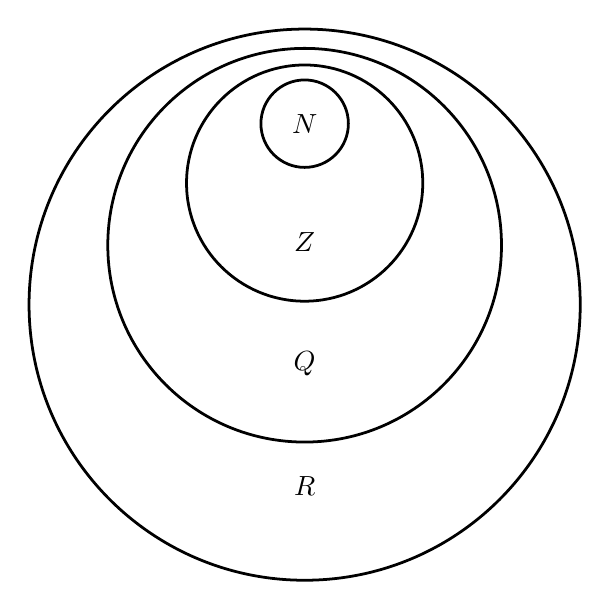
\begin{tikzpicture}[line width=1pt]
                \node (n) {\(\mathbb{N}\)};
                \node [below=of n] (z) {\(\mathbb{Z}\)};
                \node [below=of z] (q) {\(\mathbb{Q}\)};
                \node [below=of q] (r) {\(\mathbb{R}\)};
                \node[shape=circle,draw=black,fit={(n)}] {};
                \node[shape=circle,draw=black,minimum size=3cm,fit={(n) (z)}] {};
                \node[shape=circle,draw=black,minimum size=5cm,fit={(n) (q)}] {};
                \node[shape=circle,draw=black,minimum size=7cm,fit={(n) (r)}] {};
                \draw (n) (z) (q) (r);
            \end{tikzpicture}
        \end{center}
        \subsubsection{Axiomas de cuerpo}
        El conjunto de los números racionales \(\mathbb{Q}\) tiene dos operaciones: la suma o adición, y el producto o multiplicación. 
        Cada vez que sumamos o multiplicamos dos números racionales obtenemos otro racional, es decir, \(\mathbb{Q}\) es cerrado con la suma y el producto. 
        Estas dos operaciones verifican los siguientes axiomas:
        \begin{itemize}
            \item Para todo \(x\) e \(y\), \(x + y = y + x\) (la suma es conmutativa)
            \item Para todo \(x\), \(y\) y \(z\), \(x + (y + z) = (x + y) + z\) (la suma es asociativa)
            \item Existe un elemento, al que vamos a llamar cero, 0, tal que, para todo \(x\), \(x + 0 = 0 + x = x\) (existencia de elemento neutro para la suma)
            \item Para todo \(x\), existe un elemento \(z\) tal que \(x + z = z + x = 0\) (inverso para la suma)
            \item Para todo \(x\) e \(y\), \(x \cdot y = y \cdot x\) (el producto es conmutativo)
            \item Para todo \(x\), \(y\) y \(z\), \(x \cdot (y \cdot z) = (x \cdot y) \cdot z\) (el producto es asociativo)
            \item Existe un elemento, al que vamos a llamar uno, 1, tal que, para todo \(x\), \(x \cdot 1 = 1 \cdot x = x\) (existencia de elemento neutro para el producto)
            \item Para todo \(x\) distinto de 0, existe un elemento \(x^{−1}\) tal que \(x \cdot x^{−1} = x^{-1} \cdot x = 1\) (inverso para el producto)
            \item Para todo \(x\), \(y\) y \(z\), \(x \cdot (y + z) = x \cdot y + x \cdot z\) (el producto es distributivo respecto a la suma)
        \end{itemize}
        Vamos a decir que un conjunto tiene una estructura de cuerpo si es cerrado por dos operaciones que verifican los axiomas que acabamos de ver. 
        El conjunto de números reales, \(\mathbb{R}\), también es un cuerpo. Sin embargo, el conjunto de los números enteros, \(\mathbb{Z}\), no es un cuerpo ya que no verifica el ante último de los axiomas, es decir, no todos los elementos no nulos de \(\mathbb{Z}\) tienen un inverso para el producto, más aún, los únicos enteros que tienen inverso son 1 y −1.
        Una propiedad importante que tienen los cuerpos es que en ellos siempre se pueden resolver las ecuaciones del tipo \(ax + b = c\), para cualquier \(a \neq 0\) y cualquier valor de \(b\) y \(c\).
        \subsubsection{Intervalos y otros subconjuntos de la recta real}
        Un intervalo está formado por los números reales que corresponden a los puntos de un segmento o una semirrecta de la recta real. Puede incluir o no a los extremos del segmento o la semirrecta.\\
        Por ejemplo, el conjunto \(A = \{x \in \mathbb{R} / x \geq 1\}\) corresponde a los puntos de la semirrecta hacia la derecha de \(x = 1\), incluyendo a \(x = 1\):
        \begin{center}
            \begin{scaletikzpicturetowidth}{0.5\linewidth}
                \begin{tikzpicture}[scale=\tikzscale]
                    \draw [thick] (-0.1,0) -- (3.1,0);
                    \draw (0,0) node {\textbf{[}};
                    \draw (0, 0) node[below=2mm] {1};
                    \draw[line width=3mm,opacity = 0.2, blue, rounded corners] (0,0) -- (3.1, 0);
                \end{tikzpicture}
            \end{scaletikzpicturetowidth}
        \end{center}
        A este conjunto lo vamos a representar por \(A = [1, + \infty)\).
        El conjunto \(B = \{x \in \mathbb{R} / - 1 < x \leq 2\}\) corresponde a los puntos del segmento comprendido entre \(x = -1\) y \(x = 2\)
        (es decir, los puntos que se hallan a la derecha de \(x = -1\) y simultáneamente a la izquierda de \(x = 2\)), incluyendo a \(x = 2\), pero no a \(x = -1\):
        \begin{center}
            \begin{scaletikzpicturetowidth}{0.5\linewidth}
                \begin{tikzpicture}[scale=\tikzscale]
                    \coordinate (A) at (-1,0);
                    \coordinate (B) at (2,0);
                    \draw [thick] (-2.1,0) -- (3.1,0);
                    \draw (A) node {\textbf{(}};
                    \draw (B) node {\textbf{]}};
                    \draw (A) node[below=2mm] {-1};
                    \draw (B) node[below=2mm] {2};
                    \draw[line width=3mm,opacity = 0.2, blue, rounded corners] (A) -- (B);
                \end{tikzpicture}
            \end{scaletikzpicturetowidth}
        \end{center}
        En este caso, usamos la notación \(B = (-1; 2]\) para representar a este conjunto.
        \subsubsection{Cotas superiores y supremo}
        Dado un subconjunto \(A\) de números reales, decimos que un número \(K\) es \textit{cota superior} de \(A\) si en la recta todos los elementos de \(A\) están a la izquierda de \(K\). En otras palabra, si todos los elementos de \(A\) son menores o iguales que \(K\): para todo \(a \in A, a \leq K\). Podemos visualizar esta noción en la recta numérica:
        \begin{center}
            \begin{scaletikzpicturetowidth}{0.5\linewidth}
                \begin{tikzpicture}[scale=\tikzscale]
                    \draw [thick] (-1.1,0) -- (2.1,0);
                    \draw (2,0) node {\(|\)};
                    \draw[line width=3mm,opacity = 0.2, blue, rounded corners] (-.5,0) -- (1, 0);
                    \draw (2, 0) node[below=2mm] {\(K\)};
                    \draw (.25, 0) node[above=2mm] {\(A\)};
                \end{tikzpicture}
            \end{scaletikzpicturetowidth}
        \end{center}
        Si el conjunto \(A\) tiene una cota superior, decimos que \(A\) está \textit{acotado superiormente}, y la menor de todas las cotas superiores se \textit{llama supremo}.\\
        Si \(s\) es el supremo de \(A\) vamos a escribirlo \(s = sup(A)\).\\
        Demos una definición formal de supremo: si \(A\) es un conjunto de números reales, \(s\) es el supremo de \(A\) si verifica las siguientes dos condiciones:
        \begin{itemize}
            \item \(s\) es cota superior de \(A\) y
            \item si \(t\) es otra cota superior de \(A\), entonces \(s \leq t\).
        \end{itemize}
        Otra forma equivalente de definir el supremo es:
        \begin{itemize}
            \item \(s\) es cota superior de \(A\) y
            \item si \(r\) es un número real positivo cualquiera, entonces \(s - r\) no es cota superior de \(A\), es decir, siempre exite un \(a \in A\) tal que \(s - r < a \leq s\).
        \end{itemize}
        \subsubsection{Axioma de complejitud}
        Un conjunto de números reales no vacío y acotado superiormente siempre tiene supremo.\\
        El siguiente ejemplo muestra que los números racionales no verifican este axioma. Vamos a escribir \(\mathbb{R}_{>0}\) por el conjunto de los números reales estrictamente mayores que cero y \(\mathbb{Q}_{>0}\) por el de los números racionales estrictamente mayores que cero.
        \begin{center}
            \(A = \{x \in \mathbb{R}_{>0} : x^2 < 2\}\) y \(B = \{x \in \mathbb{Q}_{>0} : x^2 < 2\}\)
        \end{center}
        Ambos conjuntos, \(A\) y \(B\), son no vacíos y acotados superiormente. El número \(\sqrt{2}\) es el supremo de \(A\) ya que es la menor de las cotas superiores. Por otro lado, si nos restringimos a mirar a \(B\) dentro de los números racionales, no tiene supremo ya que toda cota superior racional de \(B\) puede ser “mejorada” por otro racional más cercano a \(\sqrt{2}\).
        \subsubsection{Cotas inferiores e ínfimo}
        En forma similar a lo desarrollado en el apartado anterior, podemos introducir las nociones de \textit{cota inferior} e \textit{ínfimo}.\\
        Una \textit{cota inferior} de un conjunto \(A \subset \mathbb{R}\) es un número \(k \in \mathbb{R}\) que es menor o igual que todo elemento de \(A\). Se dice que el conjunto \(A \subset \mathbb{R}\) está acotado inferiormente si tiene alguna cota inferior.\\
        Por ejemplo, para el intervalo \(A = (3; 7)\), algunas cotas inferiores son 2, \(\frac{5}{2}\) y 3. Por otro lado, \(\frac{1}{2}\), 1 y 2 son cotas inferiores de \(B = [2; +\infty)\), mientras que \(C = (−\infty; 5)\) no está acotado inferiormente.
        \begin{center}
            \begin{scaletikzpicturetowidth}{0.5\linewidth}
                \begin{tikzpicture}[scale=\tikzscale]
                    \coordinate (A) at (2,0);
                    \coordinate (B) at (5/2,0);
                    \coordinate (C) at (3,0);
                    \coordinate (D) at (7,0);
                    \draw [thick] (0,0) -- (8,0);
                    \draw (A) node {\(|\)};
                    \draw (B) node {\(|\)};
                    \draw (C) node {\textbf{(}};
                    \draw (D) node {\textbf{)}};
                    \draw (A) node[below=2mm] {2};
                    \draw (B) node[below=2mm] {\(\frac{5}{2}\)};
                    \draw (C) node[below=2mm] {3};
                    \draw (D) node[below=2mm] {7};
                    \draw[line width=3mm,opacity = 0.2, blue, rounded corners] (C) -- (D);
                    \draw (5,0) node[above=2mm] {\(A=(3;7)\)};
                \end{tikzpicture}
            \end{scaletikzpicturetowidth}
        \end{center}
        \begin{center}
            \begin{scaletikzpicturetowidth}{0.5\linewidth}
                \begin{tikzpicture}[scale=\tikzscale]
                    \coordinate (A) at (1/2,0);
                    \coordinate (B) at (1,0);
                    \coordinate (C) at (2,0);
                    \coordinate (D) at (8,0);
                    \draw [thick] (0,0) -- (D);
                    \draw (A) node {\(|\)};
                    \draw (B) node {\(|\)};
                    \draw (C) node {\textbf{[}};
                    \draw (A) node[below=2mm] {\(\frac{1}{2}\)};
                    \draw (B) node[below=2mm] {1};
                    \draw (C) node[below=2mm] {2};
                    \draw[line width=3mm,opacity = 0.2, red, rounded corners] (C) -- (D);
                    \draw (5,0) node[above=2mm] {\(B=[2;+\infty]\)};
                \end{tikzpicture}
            \end{scaletikzpicturetowidth}
        \end{center}
        \begin{center}
            \begin{scaletikzpicturetowidth}{0.5\linewidth}
                \begin{tikzpicture}[scale=\tikzscale]
                    \coordinate (A) at (5,0);
                    \draw [thick] (0,0) -- (8,0);
                    \draw (A) node {\textbf{)}};
                    \draw (A) node[below=2mm] {5};
                    \draw[line width=3mm,opacity = 0.2, red, rounded corners] (0,0) -- (A);
                    \draw (2.5,0) node[above=2mm] {\(C=(-\infty;5)\)};
                \end{tikzpicture}
            \end{scaletikzpicturetowidth}
        \end{center}
        Cuando un conjunto está acotado inferiormente, nos preguntamos por la ”mejor” cota inferior posible; en este caso, se trata de buscar la mayor de las cotas inferiores del conjunto. A esta última se la llama el \(\textit{ínfimo}\) del conjunto. Si \(i\) es el ínfimo de un conjunto \(A\), escribimos \(i = inf(A)\) y si el ínfimo del conjunto \(A\) pertenece a \(A\) lo llamamos \(\textit{mínimo}\).\\
        Por ejemplo, para los conjuntos \(A = (3; 7)\), \(B = [2; +\infty)\) y \(C = (−\infty; 5)\) representados en la figura de arriba, tenemos que \(inf(A) = 3\), \(inf(B) = 2\) y C no tiene ínfimo.\\
        Si \(A \subset \mathbb{R}\) es un conjunto no vacío y acotado inferiormente, el ínfimo de \(A\) es la mayor de las cotas inferiores de \(A\); en otras palabras, es un número \(i \in \mathbb{R}\) que cumple las dos condiciones siguientes:
        \begin{itemize}
            \item \(i\) es una cota inferior de \(A\),
            \item si \(d\) es una cota inferior de \(A\), entonces \(d \leq i\).
        \end{itemize}
        Al igual que con el supremo de un conjunto, hay otra forma equivalente de definir el ínfimo de un conjunto \(A: i \in \mathbb{R}\) es el ínfimo del conjunto \(A\) si
        \begin{itemize}
            \item \(i\) es una cota inferior de \(A\),
            \item para cualquier \(r\) real positivo, existe un elemento \(a \in A\) tal que \(i \geq a \geq i + r\).
        \end{itemize}
    \subsection{Funciones}
        Una función \(f: A \rightarrow B\) es una relación entre dos conjuntos, donde cada elemento del conjunto \(A\) señala un sólo elemento del conjunto \(B\).
        \begin{center}
            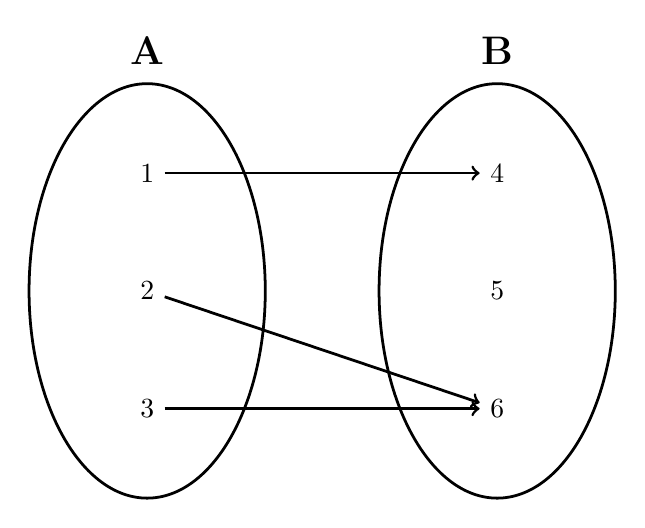
\begin{tikzpicture}[line width=1pt]
                \node (a1) {1};
                \node[below=of a1] (a2) {2};
                \node[below=of a2] (a3) {3};
                \node[right=4cm of a1] (b1) {4};
                \node[below=of b1] (b2) {5};
                \node[below=of b2] (b3) {6};
                \node[shape=ellipse,draw=black,minimum size=3cm,fit={(a1) (a3)}] {};
                \node[shape=ellipse,draw=black,minimum size=3cm,fit={(b1) (b3)}] {};
                \node[above=1cm of a1,font=\Large\bfseries] {A};
                \node[above=1cm of b1,font=\Large\bfseries] {B};
                \draw[->] (a1) -- (b1);
                \draw[->] (a2) -- (b3);
                \draw[->] (a3) -- (b3);
            \end{tikzpicture}
        \end{center}
        Se puede evaluar la función así:
        \begin{center}
            \begin{tabularx}{\textwidth}{XXX}
                \centering{\(f(1) = 4\)} & \centering{\(f(2) = 6\)} & \centering{\(f(3) = 6\)}\\
            \end{tabularx}
        \end{center}
        Como se puede ver, siempre hay un resultado por cada evaluación, no importa si hay dos o más elementos del conjunto \(A\) cuya evaluación tenga el mismo resultado.\\
        En caso contrario, no sería una función, sería una relación no funcional, como el siguiente ejemplo:
        \begin{center}
            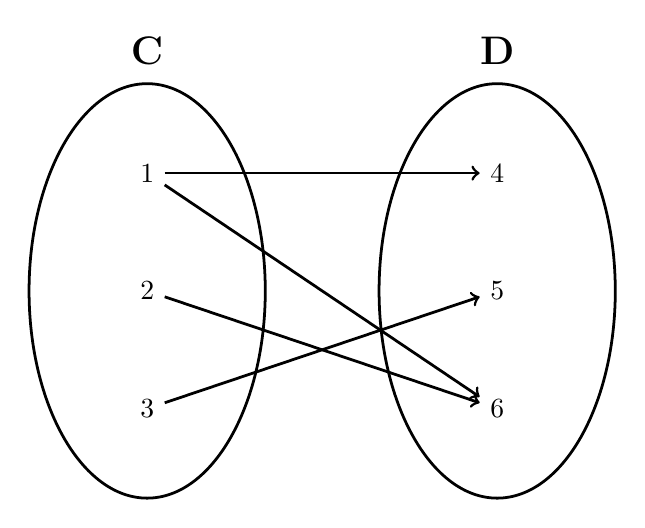
\begin{tikzpicture}[line width=1pt]
                \node (a1) {1};
                \node[below=of a1] (a2) {2};
                \node[below=of a2] (a3) {3};
                \node[right=4cm of a1] (b1) {4};
                \node[below=of b1] (b2) {5};
                \node[below=of b2] (b3) {6};
                \node[shape=ellipse,draw=black,minimum size=3cm,fit={(a1) (a3)}] {};
                \node[shape=ellipse,draw=black,minimum size=3cm,fit={(b1) (b3)}] {};
                \node[above=1cm of a1,font=\Large\bfseries] {C};
                \node[above=1cm of b1,font=\Large\bfseries] {D};
                \draw[->] (a1) -- (b1);
                \draw[->] (a2) -- (b3);
                \draw[->] (a1) -- (b3);
                \draw[->] (a3) -- (b2);
            \end{tikzpicture}
        \end{center}
        Volviendo a las funciones, a todo conjunto de salida se lo denomina el Dominio de una función, en este caso:
        \begin{center}
            \(Dom f = A\)
        \end{center}
        Por su parte, al conjunto de llegada se lo llama el Codominio de una función:
        \begin{center}
            \(Codom f = B\)
        \end{center}
\end{document}